\section{Evaluation of Virtualization vs Containerization}

\subsection{Qualitative Comparison}
	
\begin{flushleft}
Two competing technologies provide virtual resources to run NFV workloads – Virtual Machines and Containers. [1] (TABLE 1) provides a qualitative comparison of these technologies. Below table [Table 1] is an expansion of the same.

\begin{longtable}[t!]{|p{4cm}|p{4cm}|p{4cm}|}
	
\hline\hline
\textbf{Feature} & \textbf{Virtualization} & \textbf{Containerization} \\
\hline\hline
\hline
Compute Virtualization & Hardware Abstraction & Application Binary Interface \\
\hline
Interaction with the System & Hypervisor-based & System Calls \\
\hline
Base Workload & Complete Guest OS & Processes and Dependencies \\
\hline
Provisioning & Slow and Complex & Fast and Scalable \\
\hline
Resource Consumption & High & Low \\
\hline
Isolation & Full Isolation & Process-Level Isolation \\
\hline
Management & Openstack, AWS, Azure, GCE & Kubernetes, Docker Swarm, Mesos \\
\hline
Single Independent Abstraction & VM Instances & Multi-container PODs \\
\hline\hline
\label{tab:tab3}
\caption{Qualitative comparison of Virtualization and Containerization. (TABLE1 \cite[p.1663]{taleb17}}
\end{longtable}
	
\end{flushleft}

\subsection{Quantitative Comparison}

\begin{flushleft}
The differentiating factors that aids the decision of using either virtual machines or containers for running the workloads for the desired application depends on the key performance parameters. For use-cases including NFV for telecommunication services and Edge computing applications, the following performance factors are considered important:
\end{flushleft}

\begin{enumerate}
    \item Latency
    \item Throughput
    \item Isolation
    \item Allocation
\end{enumerate}

A table comparing Virtual Machines and Containers on some of the performance parameters is shown below and we can arrive at a Kiviat diagrams that represents such a table.
The comparison is made on the basis of two measures:
\begin{enumerate}
    \item Memory Sizes
    \item Running Time
\end{enumerate}


\begin{longtable}[t!]{|p{0.2\textwidth}|p{0.2\textwidth}|p{0.2\textwidth}|}
\hline\hline
Workload Description&Virtual Machines&Containers\\
\hline\hline
\hline
Kernel Compilation Memory Size (in GB)&4.0&0.42\\
\hline
MySQL Image size(in GB)&1.68&0.37\\
\hline
Memory Intensive YCSB&4.0&4.0\\
\hline
CPU Intensive SpecJBB&4.0&1.7\\
\hline
Disk Intensive Filebench&4.0&2.2\\
\hline
\hline\hline
\label{tab:tab4}
\caption{Operational memory size comparison for VMs and Containers \cite{sharma16}}
\end{longtable}

%\begin{tikzpicture}

%\tkzKiviatDiagram[scale=1.0,label distance=3cm,radial=10,gap=0.5,lattice=10]
%	{Kernel Compilation,MySQL Image,Memory Intensive,CPU Intensive,Disk Intensive}
%\tkzKiviatLine[ultra thick,color=green,mark=ball,mark size=4pt,
%               fill=green!20,opacity=0.5](4.0,1.68,4.0,4.0,4.0)
%\tkzKiviatLine[ultra thick,color=red,mark=ball,mark size=4pt,
%               fill=red!20,opacity=0.5](0.42,0.37,4.0,1.7,2.2)
%\tkzKiviatGrad[prefix=,unity=0.5](0.5)

%\end{tikzpicture}

\begin{figure}[h!]
    \centering
    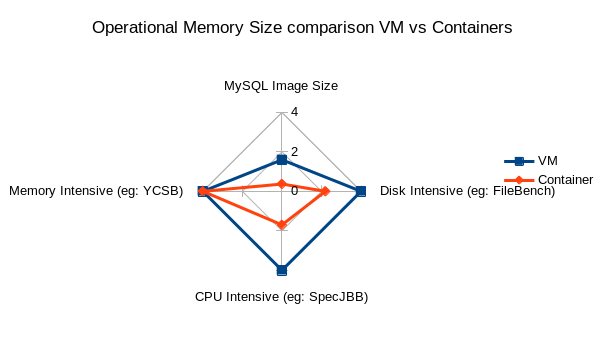
\includegraphics[width=10cm,height=6cm]{memory_size_vm_container}
    \label{fig:12}
    \caption{Comparing VMs and Containers on operational memory size, inspired from \protect\cite{mach17}}
\end{figure}

\begin{longtable}[t!]{|p{0.2\textwidth}|p{0.2\textwidth}|p{0.2\textwidth}|}
\hline\hline
\textbf{Workload Description}&\textbf{Virtual Machines}&\textbf{Containers}\\
\hline\hline
\hline
MySQL Image build Time(in sec)&236.2&129\\
\hline
Workload running time (Dist upgrade in sec)&391&470\\
\hline
Workload kernel Install(in sec)&303&292\\
\hline
\hline\hline

\label{tab:tab5}
\caption{Running time comparison for various actions for VMs and Containers \cite{sharma16}}
\end{longtable}

%\begin{tikzpicture}

%\tkzKiviatDiagram[scale=0.01,label distance=3cm,radial=10,gap=1,lattice=10]
%	{MySQL Image Build,Dist Upgrade,Kernel Install}
%\tkzKiviatLine[ultra thick,color=green,mark=ball,mark size=4pt,
%               fill=green!20,opacity=0.5](236,391,303)
%\tkzKiviatLine[ultra thick,color=red,mark=ball,mark size=4pt,
%               fill=red!20,opacity=0.5](129,470,292)
%\tkzKiviatGrad[prefix=,unity=50](50)

%\end{tikzpicture}

\begin{figure}[h!]
    \centering
    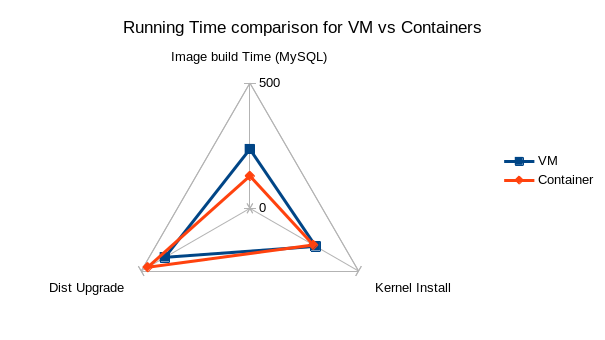
\includegraphics[width=10cm,height=6cm]{time_comparison_vm_container}
    \label{fig:13}
    \caption{Comparison of Running times for activities for VMs vs Containers \protect\cite{mach17}}
\end{figure}
